\chapter{Introduction}
\label{sec:Introduction}
One of \ippl 's most attractive features is its high performance on both single-processor and distributed-memory multiprocessor machines. As future releases of the library will also support shared-memory machines. 

The heart of the problem \ippl 's authors face is that while data-parallel programming is a natural way to express many scientific and numerical algorithms, straightforward implementations of it do exactly the wrong thing on modern architectures, whose performance depends critically on the re-use of data loaded into cache. If a program evaluates A+B+C for three arrays A, B, and C by adding A to B, then adding C to that calculation's result, performance suffers both because of the overhead of executing two loops instead of one, but also (and more importantly) because every value in the temporary array that stores the result of A+B has to be accessed twice: once to write it, and once to read it back in. As soon as this array is too large to fit into cache, the program's performance will drop dramatically.

%The first section of this tutorial explains what \ippl  does to solve this problem. Subsequent sections discuss other advanced aspects of \ippl , such as how to build pointwise functions, or reduction functions that will execute efficiently regardless of how arrays are laid out in memory.

%\ippl  tries to resolve the tension between how programmers want to express their ideas, and what runs most efficiently on modern architectures, by delaying the evaluation of expressions until enough is known about their context to ensure that they can be evaluated efficiently. It does this by blocking calculations into units called iterates, and putting those iterates into a queue of work that is still to be done. Each iterate is a portion of a computation, over a portion of a domain. \ippl  tracks data dependencies between iterates dynamically to ensure that out-of-order computation cannot occur.

%Depending on the switches specified during configuration when the library is installed, and the version of the \ippl  library that a program is linked against, \ippl  will run in one of four different modes. In the first mode, the work queue doesn't actually exist. Instead, the single thread of execution in the program evaluates iterates as soon as they are "enqueued", i.e. work is done immediately. The result is that all of the calculations in a statement are completed by the time execution reaches the semi-colon at the end of that statement.

%In its second mode, \ippl  maintains the work queue, but all work is done by a single thread. The queue is used because the explicit parceling up of work into iterates gives \ippl  an opportunity to re-order or combine those iterates. While the overhead of maintaining and inspecting the work queue can slow down operations on small arrays, it makes operations on large arrays much faster.

%For example, consider the four function calls that perform red/black relaxation in the second tutorial. In order to get the highest possible performance out of the cache, all four of these expressions should be evaluated on a given cache block before any of the expressions are evaluated for the next cache block. Managing this by hand is a nightmare, both because cache size varies from machine to machine (even when those machines come from the same manufacturer), and because very slight changes in the dimensions of arrays can tip them in or out of cache. \ippl 's array classes and overloaded operators do part of the job by creating appropriately-sized iterates; its work queue does the rest of the job by deciding how best to evaluate them. The net result is higher performance for less programmer effort.

%\ippl 's third and fourth modes of operation are multi-threaded. Each thread in a pool takes iterates from the work queue when and as they become available. Iterates are evaluated independently; the difference between the two modes is that one is synchronous, and blocks after evaluating each data-parallel statement, while the other is asynchronous, i.e. permits out-of-order execution. The table below summarizes these four modes, along with the configuration arguments used to produce each.


\section{Example 1 Laplace solver using Jacobi iteration}
\begin{code}[caption={Laplace solver}]
#include "Ippl.h"
int main(int argc, char *argv[])
{
    Ippl ippl(argc,argv);
    Inform msg(argv[0]);
    const unsigned N=8;
    const unsigned Dim=2;

    Index IGLOBAL(N);  // Specify the global domain 
    Index JGLOBAL(N); 

    Index I(1, N-1); // Specify the interior domain
    Index J(1, N-1);
    FieldLayout<Dim> layout(IGLOBAL,JGLOBAL);
    GuardCellSizes<Dim> gc(1);
    typedef UniformCartesian<Dim> Mesh;
    Field<double,Dim,Mesh> A(layout,gc);
    Field<double,Dim,Mesh> b(layout,gc);

    assign(A,0.0);  // Assign initial conditions
    assign(b,0.0);

    b[N/2][N/2] = -1.0;  // put a spike on the RHS 
    double fact = 0.25;

    // Iterate 200 times
    for (int i=0; i<200; ++i) {
        assign(A[I][J],fact*(A[I+1][J] +
                             A[I-1][J] +
                             A[I][J+1] +
                             A[I][J-1] - b[I][J]));
    }                                                                                                                                            
    msg << A << endl;
    return 0;
}
\end{code}
The syntax is very similar to that of Fortran 90: a single assignment fills an entire array with a scalar value, subscripts express ranges as well as single points, and so on. In fact, the combination of C++ and \ippl provides so many of the features of Fortran 90 that one might well ask whether it wouldn't better to just use the latter language straight up. One answer comes down to economics. While the various flavors of Fortran are still used in scientific computing, Fortran's user base is shrinking, particularly in comparison to C++. Networking, graphics, database access, and operating system interfaces are available in C++ programmers long before they're available in Fortran (if they become available at all). What's more, support tools such as debuggers and memory inspectors are primarily targeted at C++ developers, as are hundreds of books, journal articles, and web sites.

Another answer is that the abstraction facilities of C++ are much more powerful that those in Fortran. While Fortran 90 supports an attractive array syntax for floating point arrays one could not, for example, efficiently extend this high level syntax to arrays of vectors or tensors. Until recently, Fortran has had two powerful arguments in its favor: legacy applications, and performance. However, the importance of the former is diminishing as the invention of new algorithms force programmers to rewrite old codes, while the invention of techniques such as {\it expression templates} has made it possible for C++ programs to match, or exceed, the performance of highly-optimized Fortran 77. 
%!TEX encoding = UTF-8 Unicode

\section{Example 2 Power Spectrum}
A sinussoidal field  $\rho(i,j,k) = a_1sin(k_1 \frac{2\pi}{n_x} i) + a_5 sin(k_5 \frac{2\pi}{n_x} i)$, 
$i= 1 \dots n_x, ~ j= 1 \dots n_y, ~ k= 1 \dots n_z $ with $n_x,n_y$ and $n_z$ denoting the grid size is generated and
the power spectrum calculated. This examples shows how to initialise fields, compute discrete complex-complex FFT and 
compute the resulting powerspectrum.

Assume a real density field is defined like 
\begin{smallcode}
typedef Field<double,Dim,Mesh_t,Center_t>  Field_t;
Field_t rho;
\end{smallcode}
we then can immediately initialize the field according to the above formula 
\begin{smallcode}
assign(rho[I][J][K], a1*sin(2.0*pi/nr_m[0]*k1*I) + 
                     a5*sin(2.0*pi/nr_m[0]*k5*I));
\end{smallcode}
Normalizing to $\max(\rho) \le 1.0 $ with
\begin{smallcode}
rho /= max(rho)
\end{smallcode} 
we then assume to have defined a complex field "fC" and a complex-complex FFT. 
\begin{smallcode}
fC = rho;
fft->transform("forward" , fC);
 \end{smallcode}
Here we used the in place version of the FFT to obtain $\rho $ in Fourier space. Now
we can compute the power spectrum: 
\begin{smallcode}  
pwrSpec = real(fC*conj(fC));
\end{smallcode}
%\pagebreak
and calculate the 1D pwr-spectrum (in x direction) by integrating over y and z: \\
\begin{code}  
 NDIndex<3> elem;  
 for (int i=lDomain[0].min(); i<=(lDomain[0].max()-1)/2; ++i) {
  elem[0]=Index(i,i);
   for (int j=lDomain[1].min(); j<=(lDomain[1].max()-1)/2; ++j) {
    elem[1]=Index(j,j);
     for (int k=lDomain[2].min(); k<=(lDomain[2].max()-1)/2; ++k) {
       elem[2]=Index(k,k);
       f1D[i] += pwrSpec.localElement(elem);
     }
   }
 }
\end{code}
The power spectra of the local domain is stored in $f1$. We have to update all other node
so that each node has the full power spectrum by:
\begin{smallcode} 
reduce(&(f1[0]),&(f1[0])+f1_lenght,OpAddAssign());
\end{smallcode} 
assuming the non local part of $f1$ is initialized with zero.

%The full code pwrspec-1.cpp is located at $\ippl_ROOT/test/simple.

 
 \section{Example 3 Particle in Cell Code (PIC)}
 This example discusses how to write a 3D Particle in Cell Code (PIC). The 
 complete source file can be found at {\em \$IPPL\_ROOT/test/particles}. The 
 this presentation details are omitted, only the structure and important issues are
 highlighted. 
 \subsection{The {\em ChargedParticles} Class}
 The base class {\tt ParticleBase} is augmented with attributes such as charge to mass ration
 {\tt qm}, the vector momenta {\tt P} and the vector holding the electric field {\tt E}. 
 \begin{code}
 ChargedParticles(PL* pl, Vector_t hr, Vector_t rmin, 
                  Vector_t rmax, e_dim_tag decomp[Dim]) :
                  ParticleBase<PL>(pl),
                  hr_m(hr),
                  rmin_m(rmin),
                  rmax_m(rmax),
                  fieldNotInitialized_m(true)
{
    this->addAttribute(qm);
    this->addAttribute(P);
    this->addAttribute(E);

    for (int i=0; i < 2*Dim; i++) {
        this->getBConds()[i] = ParticlePeriodicBCond;
        bc_m[i]  = new PeriodicFace<double  ,Dim,Mesh_t,Center_t>(i);
        vbc_m[i] = new PeriodicFace<Vector_t,Dim,Mesh_t,Center_t>(i);
    }
    for(int i=0; i<Dim; i++)
        decomp_m[i]=decomp[i];
}
\end{code}
The arrays {\tt bc\_m} and {\tt vbc\_m} holding the boundary conditions for particles and fields.
In {\tt decomp\_m} the domain decomposition is stored.

\subsection{The {\em main}}

 \begin{code}
int main(int argc, char *argv[]) {
    Ippl ippl(argc, argv);
    Inform msg(argv[0]);

    Vektor<int,Dim> nr(atoi(argv[1]),atoi(argv[2]),atoi(argv[3]));

    const unsigned int totalP = atoi(argv[4]);
    const int nt              = atoi(argv[5]);

    e_dim_tag decomp[Dim];
    int serialDim = 2;

    Mesh_t *mesh;
    FieldLayout_t *FL;
    ChargedParticles<playout_t>  *partBunch;

    NDIndex<Dim> domain;
    for(int d=0; d<Dim; d++) {
        domain[d] = domain[d] = Index(nr[d] + 1);
        decomp[d] = (d == serialDim) ? SERIAL : PARALLEL;
    }
\end{code}
In the fist part of main, the discrete computational domain ({\tt domain}) and the 
domain decomposition ({\tt decomp}) is constructed. We have choose a 2D domain decomposition
with $z$ serial i.e. not parallelized. \\
\begin{code}
    mesh          = new Mesh_t(domain);
    FL            = new FieldLayout_t(*mesh, decomp);
    playout_t* PL = new playout_t(*FL, *mesh);

    Vector_t hr(1.0);
    Vector_t rmin(0.0);
    Vector_t rmax(nr);

    partBunch=new ChargedParticles<playout_t>(PL,hr,rmin,rmax,decomp);
\end{code} 
 Here we construct the {\tt mesh} the field layout ({\tt FL}), describing how the fields are distributed
  and finally the particle layout {\tt PL}. The latter is the used as a template argument to construct the
  particle container. For this example the mesh size is set to unity and the computational domain is
  the given by the number of mesh points defined in {\tt nr}. \\
\begin{code}
    unsigned long int nloc = totalP / Ippl::getNodes();

    partBunch->create(nloc);
    for (unsigned long int i = 0; i< nloc; i++) {
        for (int d = 0; d<Dim; d++)
            partBunch->R[i](d) =  IpplRandom() * nr[d];
    }

    partBunch->qm =  1.0/totalP;
    partBunch->myUpdate(); 
    partBunch->initFields();
\end{code} 
  Now each node created {\tt nloc} particles and initialized the coordinates randomly in the 
  computational domain.  A fixed charge to mass ration is assigned. The \texttt{myUpdate()} moves
  all particles to their node defined by the domain decomposition and initialized the fields. In the last
  call the fields gets initialized with the sinusoidal electric field.
  \clearpage
\begin{code}
    for (unsigned int it=0; it<nt; it++) {

        partBunch->R = partBunch->R + dt * partBunch->P;
        partBunch->myUpdate();
        partBunch->gather();
        partBunch->P += dt * partBunch->qm * partBunch->E;
    }
    return 0;
}
\end{code}
The last part of main consists of a simple integration scheme to advance the particles. The call
{\tt gather} interpolates the electric field at the particle position form the nearby grid points by a second
order {\it cloud in cell} (CIC) interpolation scheme. 
 
 
\subsection{{\em initFields}}
 
\begin{code}
void initFields() {

    NDIndex<Dim> domain = getFieldLayout().getDomain();

    for(int i=0; i<Dim; i++)
        nr_m[i] = domain[i].length();

    int nx = nr_m[0]; int ny = nr_m[1]; int nz = nr_m[2];

    double phi0 = 0.1*nx;            

    Index I(nx), J(ny), K(nz);

    assign(EFD_m[I][J][K](0), 
            -2.0*pi*phi0/nx * 
            cos(2.0*pi*(I+0.5)/nx) * 
            cos(4.0*pi*(J+0.5)/ny) * cos(pi*(K+0.5)/nz));

    assign(EFD_m[I][J][K](1),  ..... ;

    assign(EFD_m[I][J][K](2),  ..... ;

    assign(EFDMag_m[I][J][K],
           EFD_m[I][J][K](0) * EFD_m[I][J][K](0) +
           EFD_m[I][J][K](1) * EFD_m[I][J][K](1) +
           EFD_m[I][J][K](2) * EFD_m[I][J][K](2));
}
\end{code}

\subsection{{\em myUpdate}}
 
 \begin{code}
void myUpdate() {

    if(fieldNotInitialized_m) {
         fieldNotInitialized_m=false;
         getMesh().set_meshSpacing(&(hr_m[0]));
         getMesh().set_origin(rmin_m);
         EFD_m.initialize(getMesh(), getFieldLayout(), GuardCellSizes<Dim>(1), vbc_m);
         EFDMag_m.initialize(getMesh(), getFieldLayout(), GuardCellSizes<Dim>(1), bc_m);
    }
    this->update();  
}
\end{code}
 
  \subsection{{\em gather}}
 
\begin{code}
void gather() {	
    IntCIC myinterp;
    E.gather(EFD_m, this->R, myinterp);
}
\end{code}
 
 \section{Example 4 A Particle Particle - Particle Mesh (P$^3$M) Solver}
 Particle Particle - Particle Mesh solvers take the close range interaction of particles
into account by combining a mesh solver as seen in the previous section with a quadratic
Particle Particle computation for particles that are closer than a given interaction
radius $r_i$ (see \url{http://en.wikipedia.org/wiki/P3M}, 
\url{http://arxiv.org/abs/astro-ph/9805096} and \url{http://arxiv.org/abs/astro-ph/0512030}).
To be able to combine these two solutions the Greens functions of the PIC solver and the
particle-particle interaction have to be modified such that they add up to the desired
Green function:

\begin{equation}
G(x) = G_{pp}(x) + G_{mesh}(x).
\end{equation}
In case of the Green function $G(x) = {1 \over ||x||^2}$ this can be achieved by setting
\begin{equation}
G_{mesh}(x) = \left\{\begin{array}{cl} G(x), & \mbox{if } ||x||>r_i\\ -{3||x||^2\over r_i^4} + {4||x||\over r_i^3}, & \mbox{else} \end{array}\right.
\end{equation}
and
\begin{equation}
G_{pp}(x) = G(x) - G_{mesh}(x)
\end{equation}
see also Figure \ref{greensfunction}.

\begin{figure}[h!]
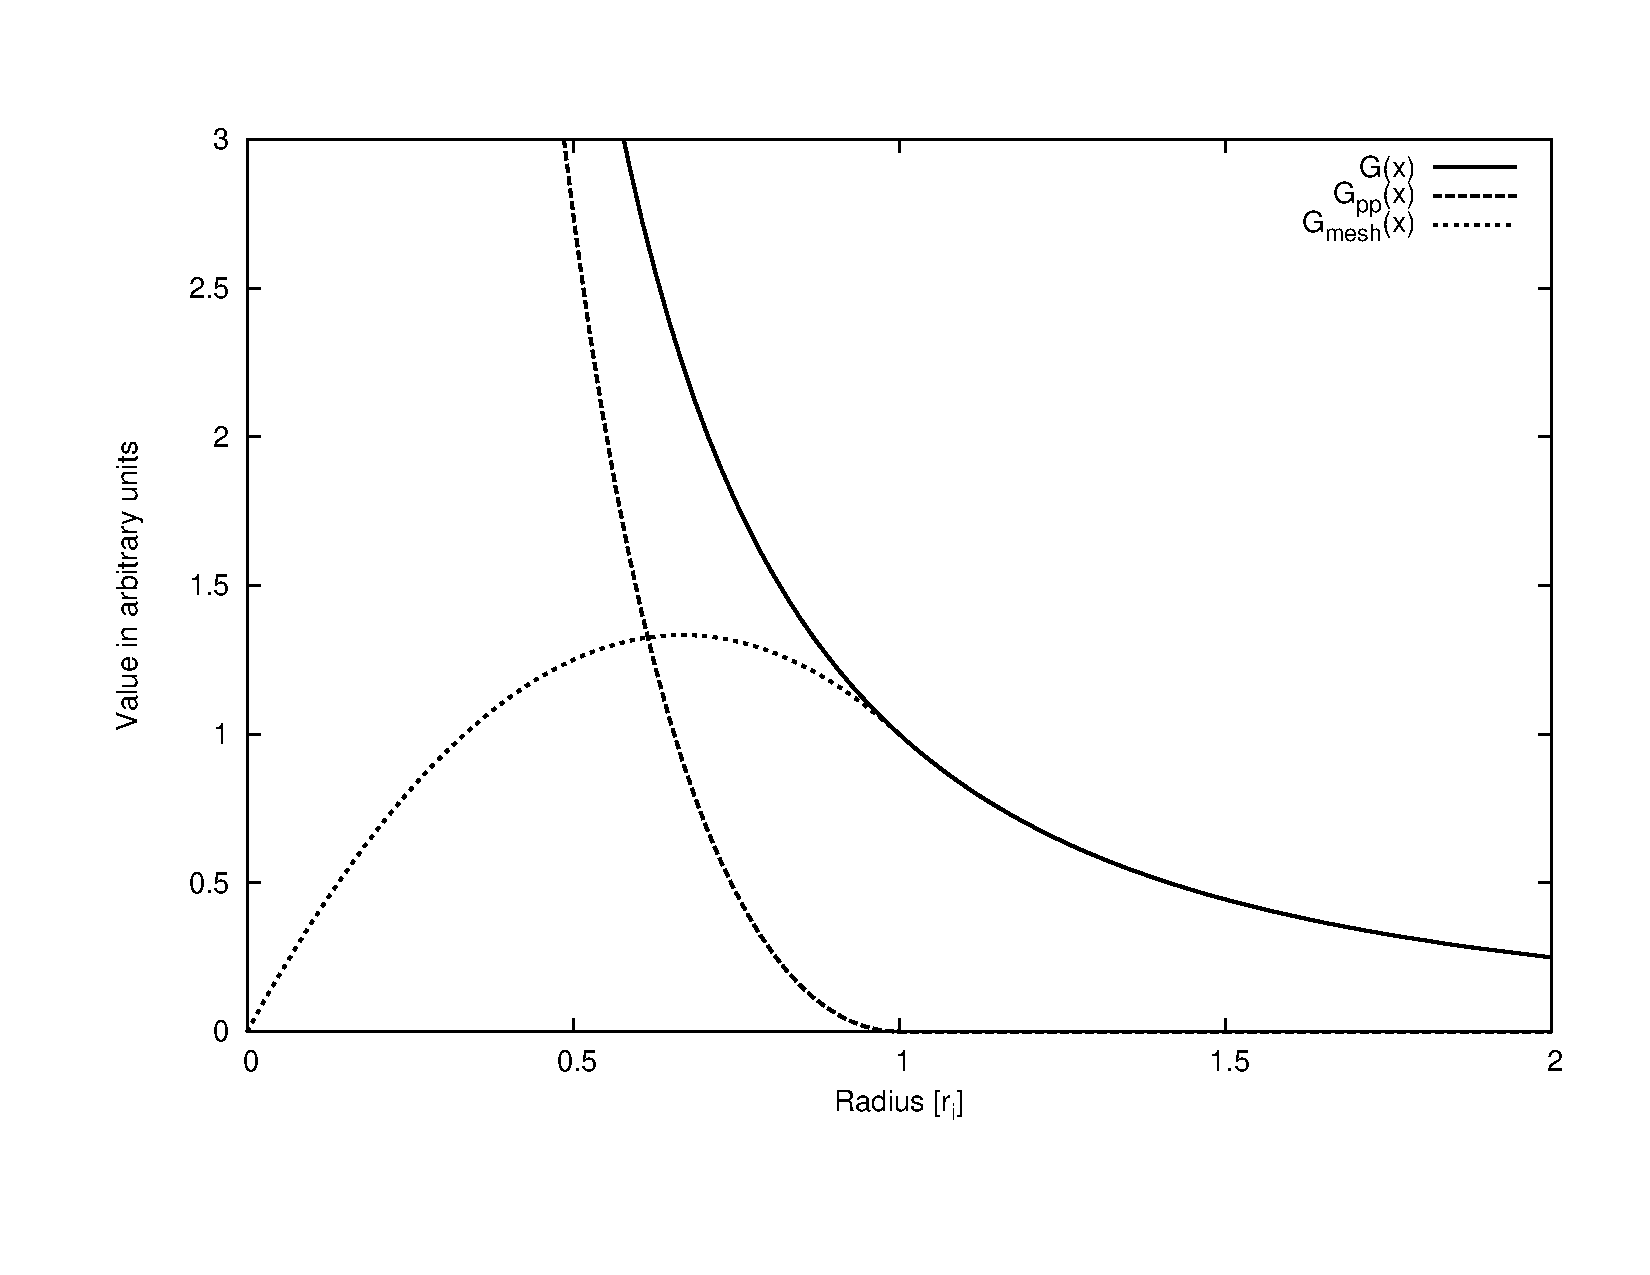
\includegraphics[width=\textwidth]{greens}
\caption{Decomposition of the Green function.}
\label{greensfunction}
\end{figure}

\begin{figure}[h!]
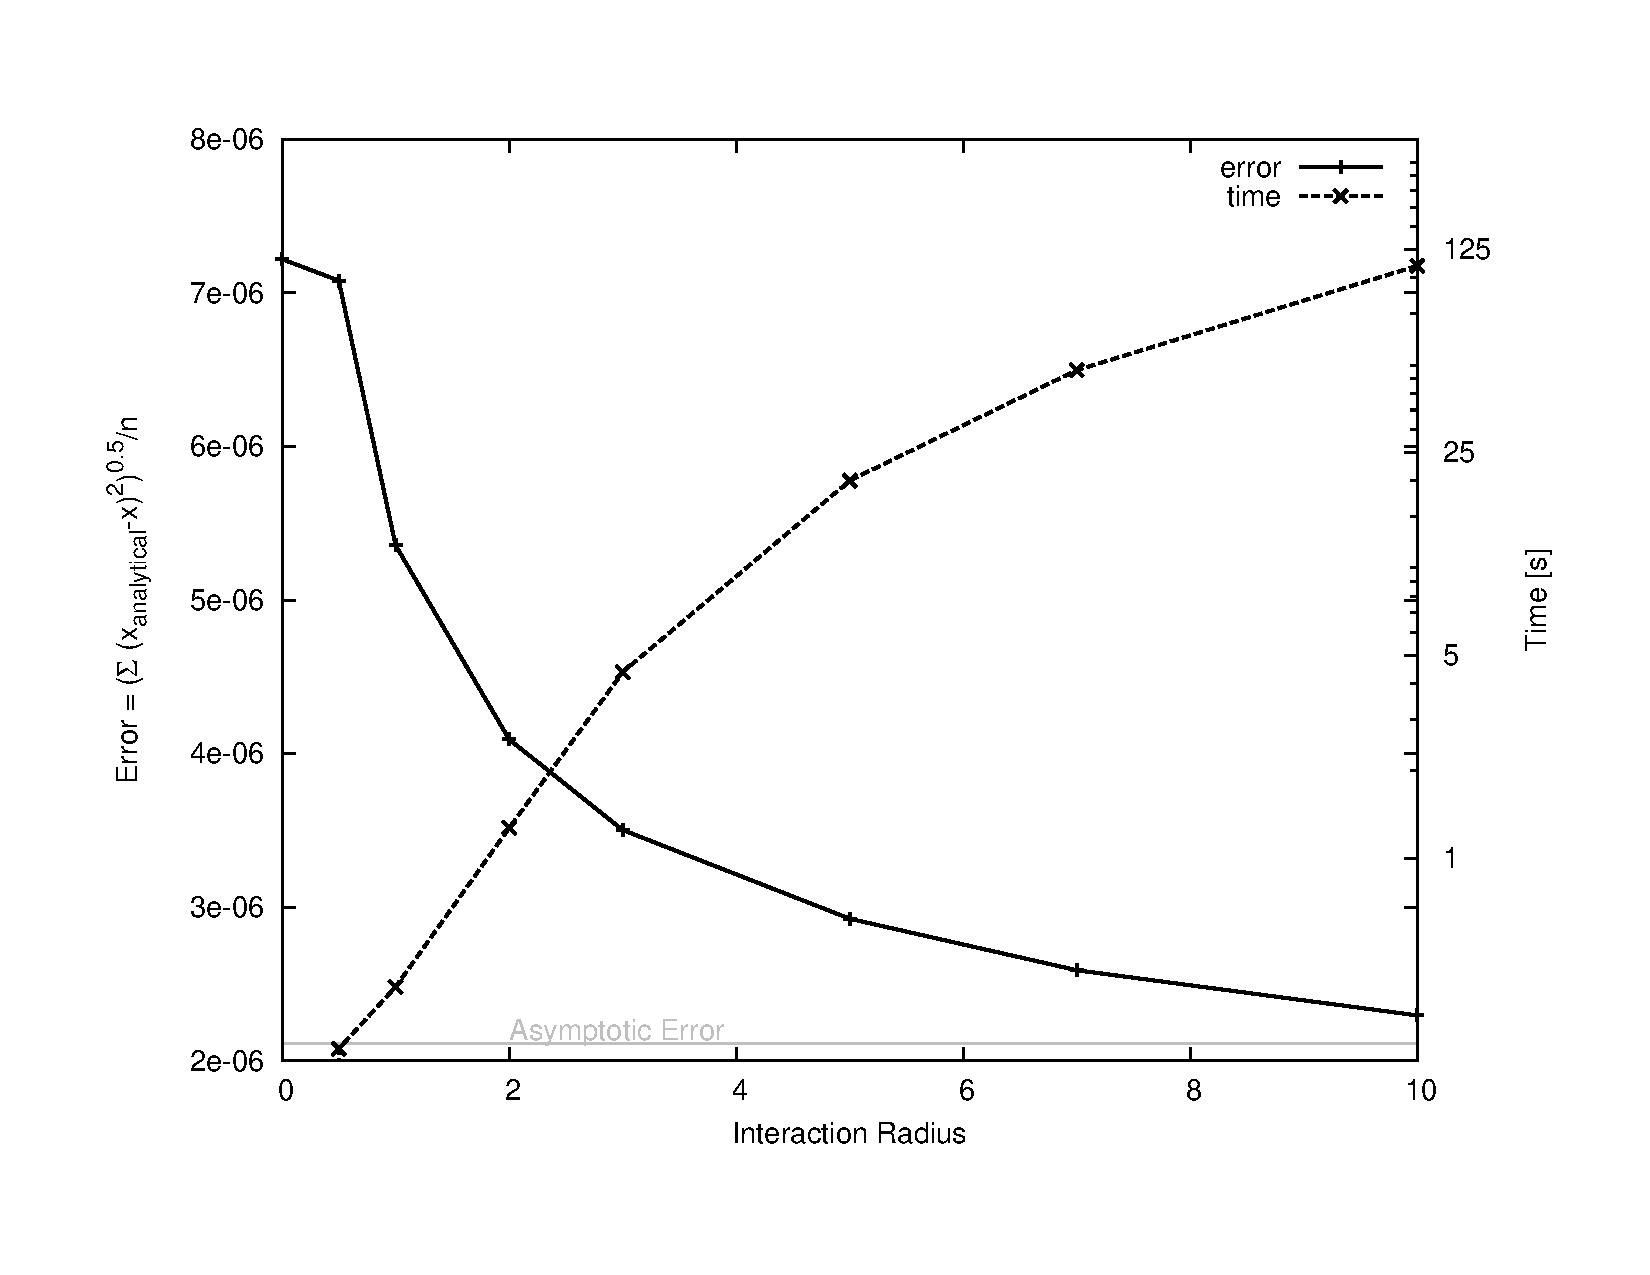
\includegraphics[width=\textwidth]{error_time}
\caption{Error and time scaling of the $P^3M$ solver for different interaction radii. Measured fo a uniform spherical
distribution of $10^4$ particles on 4 processors.}
\label{errortime}
\end{figure}
\pagebreak
Therefore the Green function from the PIC example has to be replaced by the following modified Green function:


\vspace{5mm}
\begin{code}
template<>
struct SpecializedGreensFunction<3> {
  template<class T, class FT, class FT2>
  //...

  template<class T, class FT, class FT2>
  static void calculate(Vektor<T, 3> &hrsq, FT &grn, FT2 *grnI, double R) {
    grn = grnI[0] * hrsq[0] + grnI[1] * hrsq[1] + grnI[2] * hrsq[2];
    grn = where(lt(R*R, grn), 1./sqrt(grn),
		((grn*sqrt(grn))/R-2*grn)/(R*R*R) + 2/R);
    grn[0][0][0] = grn[0][0][1];
  }   
};
\end{code}
\vspace{5mm}
The short range interaction is handled by IPPL's pairbuilding mechanism which applies
the Green function to each pair of particles whose distance is below the
interaction radius (see \ref{ppsection}). For this purpose \texttt{ChargedParticles} contains the following member
function:


\vspace{5mm}
\begin{code}
  void calculatePairForces(double interaction_radius)
  {
    HashPairBuilder< ChargedParticles<playout_t> > HPB(*this);
    //apply the field to each pair, the -1 is the field constant
    HPB.for_each(RadiusCondition<double, Dim>(interaction_radius), 
    			   ApplyField<double>(-1,interaction_radius));
  }
\end{code}
\vspace{5mm}
Which calls \texttt{ApplyField} for each pair of particles that fulfills the condition $||x_1-x_2|| = ||x|| <r_i$.
\clearpage
\pagebreak
\vspace{5mm}
\begin{code}
template<class T>
struct ApplyField {
  ApplyField(T c, double r) : C(c), R(r) {}
  void operator()(std::size_t i, std::size_t j, ChargedParticles<playout_t> &P) const
  {
    const Vector_t diff = P.R[i] - P.R[j];
    double sqr = 0;
    for(int d = 0;d<Dim;++d)
      sqr += diff[d]*diff[d];
		
     if(sqr!=0)
      {
	double r = std::sqrt(sqr);
	
	Vector_t Fij = C*(diff/r)*(1/sqr - (-3/(R*R*R*R)*r*r + 4/(R*R*R)*r));

	P.EF[i] -= P.Q[j]*Fij;
	P.EF[j] += P.Q[i]*Fij;
      }
  }
  T C;
  double R;
};
\end{code}

\section{Installation}
 \ippl uses the {\em cmake } build philosophy.  The following environment variables must be set
\begin{verbatim}
IPPL_ROOT
\end{verbatim} 
defining where \ippl is installed.

\subsection{Building \ippl}
\begin{verbatim}
cd $IPPL_ROOT
CXX=mpicxx F77=gfortran cmake -DCMAKE_VERBOSE_MAKEFILE=OFF
-DCMAKE_INSTALL_PREFIX=~/extlib/ippl $IPPL_ROOT
\end{verbatim}


\subsection{Used Compilers and Libraries}
The supported operating systems and libraries are listed in Table \ref{tab:archlib}.
\begin{table}[h]
  \caption{Supported Architectures and needed Libraries}
  \label{tab:archlib}
  \begin{center}
    \begin{tabular}{|lcccc|}
      \hline
      Operating System & HDF5  & H5hut & Compiler & Open MPI\\
      \hline
      Linux (SL) 2.6.18 & hdf5-1.8.5 & V0.99 & GNU 4.4.x, icc11.1 & 1.4.2 \\
      Cray XTx  & hdf5-1.8.5 & V0.99 & GNU 4.4 & - \\
      \hline
    \end{tabular}
  \end{center}
\end{table}



\clearpage
\section{Acknowledgements}
The contributions of various individuals and groups are acknowledged in the relevant chapters, 
however a few individuals have or had considerable influence on the 
development, Julian Cummings, Yves Ineichen and Jakob Progsch.
Misprints and obscurity are almost inevitable in a document of this size.
Comments and {\em active contributions}  from readers are therefore most welcome.
They may also be sent to \htmladdnormallink{\texttt{andreas.adelmann@psi.ch}}{mailto:andreas.adelmann@psi.ch}.

\subsection{Citation}
Please cite \ippl in the following way:
\begin{small}
\begin{verbatim} 
@techreport{ippl-User-Guide,
title = "{The IPPL (Independent Parallel Particle Layer)
              Framework }",
author = "A. Adelmann",
institution = "Paul Scherrer Institut",
number = "PSI-PR-09-05",
year = 2009}
\end{verbatim}
\end{small}


%& OPAL \\
% & V 1.0


